\documentclass[a4paper,twoside,10pt,french]{scrartcl}
\usepackage[T1]{fontenc}
\usepackage{titlesec}
\usepackage{ulem}
\usepackage[dvipsnames]{xcolor}
\usepackage{color}
\usepackage{babel}
\usepackage{helvet}
\usepackage[utf8]{inputenc}
\usepackage[T1]{fontenc}
\usepackage{geometry}
\usepackage{graphicx}
\title{34 page 286 - C7}
\date{}
 \renewcommand*\familydefault{\sfdefault}
\geometry{a4paper}
% -------------------------------------------------------------------------------------------------
% ----------- Création des commandes de couleur pour les titres ----------
% -------------------------------------------------------------------------------------------------
\newcommand{\sectionred}[1]{{\color{red}{\uuline{\color{black}#1}}}}
\newcommand{\sectiongreen}[1]{{\color{ForestGreen}{\uuline{\color{black}#1}}}}
\newcommand{\sectionblue}[1]{{\color{NavyBlue}{\uuline{\color{black}#1}}}}
\begin{document}
\maketitle
% -------------------------------------------------------------------------------------------------
% ---------------- Modification des titres de niveau 1,2 et 3 --------------------
% -------------------------------------------------------------------------------------------------
\titleformat
{\section} % command
%[display] % shape
{\Large} % format
{{\color{red}\uuline{\color{black}}}} % label
{0ex} % sep
{\sectionred} % before-code
[] % after-code

\titleformat
{\subsection}%[display] % shape
{\Large} % format
{{\color{ForestGreen}\uuline{\color{black}}}} % label
{0ex} % sep
{\sectiongreen} % before-code
[] % after-code

\titleformat
{\subsubsection} % command
%[display] % shape
{\large} % format
{{\color{NavyBlue}\uuline{\color{black}}}} % label
{0ex} % sep
{\sectionblue} % before-code
[] % after-code

% -------------------------------------------------------------------------------------------------
% ---------------- Début du corps du document ------------------------------------
% -------------------------------------------------------------------------------------------------

\subsection{1)Altitude\:et\:énergie\:potentielle\:de\:pesanteur}
\subsubsection{a)Altitude\:en\:A\:et\:B}
On peut modéliser la situation par 2 triangles rectangles dont on connaît une longueur (L) et un angle ($\alpha$) (en plus de l'angle à 90°). On schématise :

\includegraphics{34-fig1}

Pour trouver l'altitude des 2 points, il faut chercher la longueur des segments jaune et violet.

On applique des propriétés de trigonométrie : $\cos(\alpha) = \frac{Adjacent}{Hypothénuse}$

Pour $Z_A$ : $\cos(\alpha_A) = \frac{Z_A}{L} \Leftrightarrow Z_A = \cos(\alpha_A) \times L$

Pour $Z_B$ : $\cos(\alpha_B) = \frac{Z_B}{L} \Leftrightarrow Z_B = \cos(\alpha_B) \times L$

Mais comme les points A et B sont en dessous du point O, où $E_{pp} = 0$, il faut rajouter le signe moins (-) devant chaque expression. Si on ne le faisait pas, on trouverais que $Z_A$ est plus haut que $Z_B$. Or, ce n'est pas le cas.

Finalement, on trouve : $Z_B = - \cos(\alpha_B) \times L$ et $Z_A = - \cos(\alpha_A) \times L$.
\subsubsection{b)Expression\:de\:l'énergie\:potentielle\:en\:A\:et\:B}
$E_{pp, A} = m \times g \times Z_A = m \times g \times - \cos(\alpha_A) \times L$

$E_{pp, B} = m \times g \times Z_B = m \times g \times - \cos(\alpha_B) \times L$

\subsection{2)Énergie\:mécanique}
\subsubsection{a)Expression\:de\:l'énergie\:mécanique}
$E_{m, A} = E_{pp, A} + E_{c, A}$.

Or, je sais que $E_{c, A} = \frac{1}{2}mv_A^2$ et d'après 1.b), $E_{pp, A} = m \times g \times - \cos(\alpha_A) \times L$.

Donc : $E_{m, A} = m \times g \times - \cos(\alpha_A) \times L + \frac{1}{2}mv_A^2$.

Même raisonnement pour $E_{m, B}$ : $E_{m, B} = m \times g \times - \cos(\alpha_A) \times L + \frac{1}{2}mv_B^2$.

Mais, au point B, la vitesse est nulle.

On obtient finalement pour $E_{m, B}$ : $E_{m, B} = m \times g \times - \cos(\alpha_B) \times L$.
\subsubsection{b)Calcul\:de\:l'angle\:maximum\:de\:$\alpha_B$}

Comme les frottements sont négligeables, $\Delta E_m = 0$

Or, je sais que $\Delta E_m = \Delta E_{pp} + \Delta E_c$.

Donc : $\Delta E_{pp} + \Delta E_c = 0$

Or, $\Delta E_{pp} = E_{pp, A} - E_{pp, B}$ car la boule part de B pour aller vers A.

Même raisonnement pour $\Delta E_c$.

Donc : $(E_{pp, A} - E_{pp, B}) + (E_{c, A} - E_{c, B}) = 0$

Donc : $E_{pp, A} - E_{pp, B} + E_{c, A} - E_{c, B} = 0$

On remplace les énergie potentielles et cinétiques par leurs expressions. On trouve :

$$( - m \times g \times \cos(\alpha_A) \times L) - ( - m \times g \times \cos(\alpha_B) \times L) + \frac{1}{2}mv_A^2 - \frac{1}{2}mv_B^2 = 0$$

Mais la vitesse au point B est nulle, on peut simplifier l'expression :
$$( - m \times g \times \cos(\alpha_A) \times L) - ( - m \times g \times \cos(\alpha_B) \times L) + \frac{1}{2}mv_A^2 = 0$$

On simplifie l'expression :

$$m \times g \times (-\cos(\alpha_A)) \times L + m \times g \times \cos(\alpha_B) \times L) + \frac{1}{2}mv_A^2 = 0$$

%%On factorise : $$m \times g \times ((-\cos(\alpha_A))+ \cos(\alpha_B) \times L) + \frac{1}{2}mv_A^2 = 0$$

On fait passer l'expression de l'énergie potentielle de pesanteur au point B de l'autre côté :
$$m \times g \times (-\cos(\alpha_A)) \times L + \frac{1}{2}mv_A^2 = - m \times g \times \cos(\alpha_B) \times L) $$

On peut simplifier en enlevant la masse car elle se trouve des 2 côtés de l'équation (On aurait pu le faire avant (mais j'ai oublié...)) :
$$g \times (-\cos(\alpha_A)) \times L + \frac{1}{2}v_A^2 = - g \times \cos(\alpha_B) \times L) $$

On divise par $-g \times L$ pour obtenir :

$$\cos(\alpha_A) - \frac{v_A^2}{2 \times g \times L} = \cos(\alpha_B)$$

On n'a plus qu'à faire arcos pour trouver l'angle :
$$\cos^{-1}(\cos(\alpha_A) - \frac{v_A^2}{2gL}) = \alpha_B$$

APP.N : $\alpha_B = \cos^{-1}(\cos(30) - \frac{1.0^2}{2 \times 9.81 \times 20 \cdot10^{-2}}) = 52$°.
\end{document}
